\documentclass[a4paper,12pt]{report}

\usepackage{alltt, fancyvrb, url}
\usepackage{graphicx}
\usepackage[utf8]{inputenc}
\usepackage{float}
\usepackage{xcolor}
\usepackage{hyperref}
\usepackage{ifluatex}
\ifluatex
  \usepackage{pdftexcmds}
  \makeatletter
  \let\pdfstrcmp\pdf@strcmp
  \let\pdffilemoddate\pdf@filemoddate
  \makeatother
\fi
\usepackage{svg}

\usepackage[italian]{babel}

\usepackage[italian]{cleveref}

\title{Relazione del progetto \\``Balatro-Lite''}
\author{
    Enrico Bartocetti\\
    Nicholas Benedetti\\
    Justin Carideo\\
    Nicolas Tazzieri
}
\date{\today}

\begin{document}

\maketitle

\newpage

\tableofcontents

\chapter{Analisi}

\section{Descrizione e requisiti}
Il software Balatro lite è un videogioco di carte che combina il solitario alle meccaniche del poker. Lo scopo del gioco è quello di superare diversi livelli, detti ante, di difficoltà incrementale.

Per ogni ante è necessario superare 3 round detti blind, nei quali bisogna, attraverso le combinazioni tipiche del poker e con l’aiuto di alcune carte speciali, raggiungere un determinato punteggio in chips.

In ogni round il giocatore ha a disposizione un numero di mani da giocare. Una volta esaurite, la partita si conclude e viene controllato il numero di chips raccolto. Se i chips accumulati sono inferiori al punteggio da raggiungere, il gioco termina e il giocatore perde.  

Il gioco prevede una serie di mazzi, ognuno dotato di proprietà che modificano alcuni aspetti della partita (ad esempio il numero di mani, scarti, chips).

Ogni round consiste in delle giocate nelle quali l’utente dovrà utilizzare le carte che ha in mano per fare delle combinazioni. A ogni combinazione viene attribuito un punteggio, formato da una coppia composta da punteggio base e moltiplicatore, che verrà convertito in chips. L’utente ha anche a disposizione un certo numero di scarti, con i quali può scegliere delle carte della mano da scartare.  L'ultimo blind di ogni ante è un boss, ovvero depotenzia in vari modi le mani giocate.

A fine round, se viene superato il punteggio prestabilito, l’utente verrà ricompensato con una valuta di gioco che gli permetterà di effettuare acquisti nel negozio. Il negozio viene aperto a fine round ed è possibile acquistare power up di vario tipo (ad esempio Joker).  

Le carte speciali hanno lo scopo di modificare alcuni aspetti della partita. In particolare, i Joker si occupano di modificare il punteggio base e i moltiplicatori forniti dalle combinazioni. Queste carte possono essere rivendute in qualsiasi momento del gioco.

\subsubsection{Requisiti funzionali}
\begin{itemize}
  \item Il giocatore potrà scegliere tra diversi mazzi a inizio partita, ognuno dei quali apporterà delle modifiche a ogni round.
  \item Su richiesta dell'utente dovrà essere possibile visualizzare le combinazioni disponibili durante il gioco.
  \item Dovranno essere previsti diversi Joker all’interno dello shop, che dovranno apparire con una diversa frequenza preimpostata.
  \item I modificatori dovranno essere applicati solo in determinate condizioni (ad esempio quando vengono giocate certe carte o certe combinazioni).
  \item Durante il round dovrà essere possibile ordinare le carte in mano in base al seme o al valore della carta.
\end{itemize}

\subsubsection{Requisiti non funzionali}
\begin{itemize}
	\item L’interazione con l’utente dovrà risultare fluida.
	\item L’interfaccia grafica dovrà essere ridimensionabile.
  	\item Il look and feel dovrà risultare omogeneo tra i vari sistemi operativi.
\end{itemize}

\section{Modello del Dominio}
Il gioco prevede una serie di ante, ognuno formato da diversi round detti blind.
Esistono diversi mazzi che conterranno le carte da giocare durante i vari round.
Ogni carta ha di base un seme e un valore, e dei modificatori che possono essere aggiunti col proseguire della partita.
In ogni blind il giocatore disporrà di due slot. Uno conterrà le carte del mazzo che l’utente potrà giocare e l’altro conterrà invece le carte speciali.
Ogni combinazione ha un punteggio base e un moltiplicatore: una volta giocata la mano verrà effettuato il calcolo del punteggio totale, che concorrerà al raggiungimento della soglia minima di chips per superare il blind.
Data la crescente quantità di chips necessaria al superamento del blind, sarà necessario avere delle combinazioni “più potenti”: per questo sono presenti i Joker, carte speciali che al soddisfare di certe condizioni modificano il punteggio totale della combinazione.
Alla fine di ogni round, al giocatore verrà riconosciuta una ricompensa tramite una valuta in-game e verrà visualizzato lo shop, con la quale potrà acquistare le carte speciali.

\begin{figure}[H]
	\centering{}
	\includesvg[width=1\textwidth,pretex=\tiny]{img/Analisi}
	\caption{Schema UML dell’analisi del problema, con rappresentate le entità principali ed i rapporti tra loro.}
	\label{img:analisi}
\end{figure}

\chapter{Design}

\section{Architettura}
L’architettura del gioco Balatro lite segue il pattern architetturale MVC.
Questo pattern prevedendo una divisione dei compiti tra il Modello, il Controller e la View, ci permetterà di approcciarci allo sviluppo in maniera settoriale.
Questo ci consentirà ad esempio di poter rinnovare completamente la veste grafica del gioco utilizzando dei motori grafici più avanzati senza toccare Model e Controller.

Il modello presenta 3 entry point principali:
\begin{itemize}
	\item \texttt{Player}, per poter gestire le statistiche che rimangono valide per tutto il gioco, ad esempio i soldi del giocatore, il mazzo scelto, le carte speciali.
	\item \texttt{Ante}, per poter gestire i singoli round, ad esempio la soglia di chips di ogni blind, la sua ricompensa, le carte da giocare.
	\item \texttt{Shop}, per poter gestire la vendita delle carte speciali. 
\end{itemize}
Per poterlo gestire, la nostra architettura prevede la presenza di più controller (uno per entry point del modello), coordinati da un \texttt{MasterController}. Quest’ultimo si occuperà anche della comunicazione con la \texttt{View}.
Le View possono essere agganciate al master controller tramite il metodo \texttt{attachView()}, rendendo quindi il controller capace di gestire più viste contemporaneamente. La comunicazione avviene nella seguente maniera:
\begin{itemize}
	\item Le view notificano i cambiamenti al controller chiamando il metodo \texttt{handleEvent()} del master controller specificando il relativo evento, e passando opzionalmente i dati da gestire.
	\item Il controller notifica alle view i comportamenti da attuare chiamando dei metodi appositi e scambiando le informazioni attraverso delle classi di comunicazione.
\end{itemize}
Questo ci consente di astrarre completamente la view dal model, visto che i controller si occupano di eseguire le conversioni tra la struttura dei dati contenuti nel model e quelli forniti alla view. 

La view presenta un’interfaccia contenente metodi per l’aggiornamento delle componenti grafiche, astraendola completamente dalle possibili implementazioni.
Sarà ad esempio possibile aggiungere una view ad interfaccia a linea di comando senza dover toccare né il model né il controller.

\begin{figure}[H]
	\centering{}
	\includesvg[width=1\textwidth]{img/ArchitetturaMVC}
	\caption{Schema UML del diagramma architetturale, in cui si evidenzia la separazione tra le parti di Model, View, Controller e come i controller si interfacciano col Model.}
	\label{img:architetturamvc}
\end{figure}

\section{Design dettagliato}

\subsection{Bartocetti Enrico}

\subsubsection*{Modifica delle caratteristiche di un Blind}
\begin{figure}[H]
	\centering{}
	\includesvg[width=1\textwidth,pretex=\tiny]{img/BlindModifier}
	\caption{Rappresentazione UML del pattern Strategy per i modificatori dei blind.}
	\label{img:blindmodifier}
\end{figure}
\paragraph{Problema}
Deve essere possibile modificare il numero di mani e di scarti che il giocatore ha a disposizione e il moltiplicatore da applicare ogni volta che vengono guadagnati dei chips. 
\paragraph{Soluzione}
Il sistema per la gestione dei modificatori segue il \textit{pattern Strategy}, come da \Cref{img:blindmodifier}. Ho creato l’interfaccia strategy \texttt{BlindModifier}, che mette a disposizione i tre metodi per poter calcolare i nuovi valori dati quelli vecchi.
Ogni \texttt{Blind} avrà quindi un BlindModifier, e richiamerà i suoi metodi quando necessario. L’unica implementazione è data da \texttt{BlindModifierImpl}: questa classe utilizza a sua volta strategy, poiché contiene tre \texttt{UnaryOperator}, uno per ogni algoritmo richiesto da BlindModifier.
Così facendo, essendo UnaryOperator un’interfaccia funzionale, posso crearne nuove istanze utilizzando semplicemente delle espressioni lamba. Ho preferito il pattern strategy al template method perché mi permette di avere codice molto più compatto.
Inoltre, preferisco la composizione all’ereditarietà poiché Java pone il vincolo dell’ereditarietà singola: scegliendo la composizione in futuro sarà possibile creare altri modificatori che estendono un’altra classe se necessario.

\subsubsection*{Creazione di Blind}
\begin{figure}[H]
	\centering{}
	\includesvg[width=1\textwidth,pretex=\tiny]{img/BlindFactory}
	\caption{Rappresentazione UML del pattern Abstract Factory per la creazione di Blind.}
	\label{img:blindfactory}
\end{figure}
\paragraph{Problema}
Fornire un mezzo per la creazione di Blind facendo in modo che questi siano di difficoltà differente. 
\paragraph{Soluzione}
Per fornire uno strumento per la creazione di Blind ho utilizzato il \textit{pattern Abstract Factory}, come da \Cref{img:blindfactory}.
In questo caso il ruolo di AbstractFactory è assunto dall’interfaccia \texttt{BlindFactory}, che si occupa di produrre AbstractProduct di interfaccia \texttt{Blind}.
Nella mia implementazione, la classe \texttt{BlindFactoryImpl} (ConcreteFactory) crea oggetti delle classi \texttt{BaseBlind} e \texttt{BossBlind} (ConcreteProduct).
Questo permetterà di cambiare agilmente l’implementazione dei Blind prodotti dalla factory in caso di future modifiche alle classi.
Per impostare la difficoltà (ovvero il numero minimo di chips) e la ricompensa, ho utilizzato il \textit{pattern Strategy} così che chi utilizzerà la factory deciderà le funzioni per determinare questi due parametri.
La difficoltà viene calcolata grazie a un  \texttt{BinaryOperator}, ovvero una funzione che presi il numero dell’ante di cui fa parte il blind e il numero del blind stesso, produce il numero minimo di chips necessario per superare il blind.
La ricompensa invece viene calcolata tramite l’applicazione di un  \texttt{UnaryOperator}, ovvero una funzione che preso l’id del blind produce in output la ricompensa.
Nel nostro progetto le implementazioni delle strategie non sono classi effettive, ma delle lambda essendo Unary e Binary Operator delle interfacce funzionali.
Infine, la BlindFactoryImpl deve ricevere il  \texttt{BlindModifier} che dovrà applicare ai Blind creati.

\subsubsection*{Creazione di vari Deck con modificatori}
\begin{figure}[H]
	\centering{}
	\includesvg[width=1\textwidth,pretex=\tiny]{img/BuffedDeck}
	\caption{Rappresentazione UML del sistema per la creazione di Deck.}
	\label{img:buffeddeck}
\end{figure}
\paragraph{Problema}
Il gioco deve permettere al giocatore di scegliere un mazzo da utilizzare per tutta la partita che apporterà delle modifiche a ogni blind che affronterà. Devono quindi esistere vari deck con vari modificatori.
\paragraph{Soluzione}
Per aggiungere i potenziamenti al mazzo di carte ho creato l’interfaccia  \texttt{BuffedDeck}, che estende l’interfaccia  \texttt{Deck}.
Così facendo vengono rispettati i principi \textit{KISS} (Keep It Simple, Stupid), \textit{OCP} (Open / Closed Principle) e \textit{SRP} (Single Responsibility Principle), visto che Deck si occupa solamente di gestire le carte da gioco e BuffedDeck ne aggiunge i potenziamenti.
La creazione di questi BuffedDeck avviene grazie alla classe  \texttt{BuffedDeckFactory} seguendo il \textit{pattern Simple Factory}.
Nello specifico, la factory produce oggetti \texttt{BuffedDeckImpl}, classe che ho creato estendendo l'implementazione già esistente di \texttt{DeckImpl}.
Al momento della creazione di ogni BuffedDeck viene anche creato il relativo modificatore (il cui funzionamento è stato spiegato in \Cref{img:blindmodifier}).
Il sistema è esemplificato in \Cref{img:buffeddeck}.

\subsection{Benedetti Nicholas}
L'idea di creare diversi tipi di \textit{blind} è stata applicata tramite un \textbf{refactor} di alcune classi già presenti e create da Bartocetti Enrico.

\subsubsection*{Presenza di Diversi Tipi di Blind}

\begin{figure}[H]
	\centering{}
	\includesvg[width=1\textwidth,pretex=\tiny]{img/DifferentBlind}
	\caption{UML dell'applicazione del pattern Template Method per diversi tipi di Blind}
	\label{img:differentblind}
\end{figure}

\paragraph{Problema}
Vogliamo creare diversi tipi di \textit{blind} avendo una base unica e qualche metodo da poter implementare diversamente a seconda del tipo di \textit{blind} che vogliamo creare.

\paragraph{Soluzione}
Una delle possibili soluzioni è l’utilizzo del \textbf{Template Method Pattern}. 

Ho implementato la classe \texttt{AbstractBlind} definendo quasi tutti i metodi dell’interfaccia \texttt{Blind}, tranne alcuni (quelli descritti nell’UML). Essendo questa classe astratta, risulta ora molto semplice implementare diversi tipi di \textit{blind}, come:

\begin{itemize}
    \item \textbf{BaseBlind}
    \item \textbf{BossBlind}
\end{itemize}

Ogni \textit{blind} dovrà solamente implementare i seguenti due metodi:

\begin{itemize}
    \item \texttt{evaluateChips()}: utilizzato per calcolare le \textit{chips} guadagnate dalla mano giocata, dopo aver applicato i propri \textit{modifier}.
    \item \texttt{getDescription()}: restituisce la descrizione del \textit{blind}, ovvero i suoi \textit{debuff} (se presenti).
\end{itemize}

\begin{figure}[h]
    \centering
    \caption{}
\end{figure}

\subsubsection*{Implementazione Boss Blind}

\begin{figure}[H]
	\centering{}
	\includesvg[width=1\textwidth,pretex=\tiny]{img/BossBlind}
	\caption{UML dell’implementazione del Boss Blind}
	\label{img:bossblind}
\end{figure}

\paragraph{Problema}
Creare un insieme di \textit{debuff} dal quale poterne scegliere uno randomicamente da assegnare al \textit{Boss Blind}.

\paragraph{Soluzione}
L’idea è di creare una \textbf{factory} di \textit{debuff}, implementata tramite la classe \texttt{BossModifiersCatalog}, che, attraverso metodi privati, costruisce un catalogo di \textit{debuff}. Questo catalogo viene utilizzato tramite il metodo \texttt{getRandom()}, che restituisce un \textit{debuff} casuale.

\subsubsection*{Gestione degli Slot a Livello di UI}

\begin{figure}[H]
	\centering{}
	\includesvg[width=1\textwidth,pretex=\tiny]{img/SlotPanel}
	\caption{UML implementazione SlotPanel}
	\label{img:slotpanel}
\end{figure}

\paragraph{Problema}
Il problema affrontato riguarda l'implementazione generica del concetto di \textit{slot} a livello GUI.

\paragraph{Soluzione}
L'idea è stata realizzata tramite l'implementazione della classe \texttt{SlotPanel}. Questa classe è un wrapper di un \texttt{JPanel} utilizzato per contenere un qualsiasi oggetto (in questo caso una carta). Gli oggetti vengono visualizzati come \texttt{JButton} e, tramite costruttore, è possibile definire:

\begin{itemize}
    \item \texttt{Supplier<Boolean> clickable}: definisce quando rendere il bottone cliccabile.
    \item \texttt{Supplier<Boolean> removable}: definisce la possibilità di rimuovere l'oggetto (quindi anche il bottone).
    \item \texttt{Consumer<X> consumer}: l'azione da compiere quando il bottone viene premuto.
\end{itemize}

La \textbf{rimozione} del bottone avviene di default se i test \texttt{clickable} e \texttt{removable} passano.

\subparagraph{addObject()}
Il metodo \texttt{addObject()} richiede come parametro un oggetto \texttt{SlotObject}. Questo oggetto è definito come \texttt{record} all’interno della classe \texttt{SlotPanel} e contiene:

\begin{itemize}
    \item \texttt{X obj}: l'oggetto da aggiungere.
    \item \texttt{String name}: il nome dell'oggetto.
    \item \texttt{String path}: il percorso per cercare l'immagine da mostrare.
\end{itemize}

\subsection{Carideo Justin}
\subsubsection*{Riconoscimento delle combinazioni}
\begin{figure}[H]
	\centering{}
	\includesvg[width=1\textwidth,pretex=\tiny]{img/Recognizers}
	\caption{Rappresentazione UML dei vari riconoscitori delle combinazioni}
	\label{img:recognizers}
\end{figure}
\paragraph{Problema}
Il gioco dovrà essere in grado di riconoscere le combinazioni giocate dall’utente.
\paragraph{Soluzione}
Innanzitutto si è voluto rappresentare il concetto di mano giocata attraverso la classe \texttt{PlayedHand},
al cui interno troviamo il metodo \texttt{evaluateCombination}, che dovrà restituire la soluzione.
Ho separato in due parti il sistema di riconoscimento: \texttt{CombinationRecognizer} (per riconoscere la combinazione)
e \texttt{CombinationCalculator} (per calcolarla e compattare il tutto nella classe \texttt{Combination}, questa classe verrà
trattata in seguito). In questa parte verrà trattata la prima fase di riconoscimento, dove \texttt{CombinationRecognizer} è
l’interfaccia principale da cui riconoscere le varie combinazioni.
Per risolvere questo problema ho fatto in modo che \texttt{PlayedHand} avesse una tabella di riferimento
delle varie tipologie di combinazioni con associato a ciascuno un riconoscitore. La tabella dovrà dire se la mano giocata
corrisponde (oppure no) a una determinata combinazione e nel caso ritornare la migliore fra queste.
A questo punto il problema passa alla costruzione dei vari \texttt{CombinationRecognizer} e l'implementazione dipende fortemente
dal tipo di combinazione che si vuole riconoscere.
Essendo un'implementazione di un algoritmo per ciascun tipo di combinazione, doveva essere inizialmente parte di uno \textit{Strategy} pattern, nella quale
\texttt{CombinationRecognizer} è il contesto del pattern e ciò seguiva il principio \texttt{SRP}.
Tuttavia ciò comportava un problema relativo a troppe classi da gestire perché si dovrebbe realizzare una strategia concreta
per ciascuna tipologia di combinazione; in più alcune combinazioni condividono alcune somiglianze in
termini di algoritmi. Di conseguenza ho optato per una soluzione che segue il principio DRY ed è
rappresentata dalla classe \texttt{CombinationRecognizerFactory}, come viene mostrato in \Cref{img:recognizers}.
Quest’ultima segue il pattern \textit{Factory Method}, dove il prodotto è un \texttt{CombinationRecognizer} e
\texttt{CombinationRecognizerFactory} è il produttore. Ciascun riconoscitore viene implementato come
classe anonima sfruttando il fatto che \texttt{CombinationRecognizer} è un'interfaccia funzionale.
 Una volta prodotti i vari riconoscitori, \texttt{PlayedHand} li associa alla corrispettiva
 combinazione ed è in grado di sapere quale sarà quella giusta.

 \subsubsection*{Calcolo delle combinazioni}
 \begin{figure}[H]
	 \centering{}
	 \includesvg[width=1\textwidth,pretex=\tiny]{img/Calculators}
	 \caption{Rappresentazione UML dei vari calcolatori delle combinazioni}
	 \label{img:calculators}
 \end{figure}
 \paragraph{Problema}
 Utilizzare degli algoritmi per calcolare le combinazioni in base alle carte giocate.
 \paragraph{Soluzione}
 Riprendendo il problema precedente, questa sezione parlerà della seconda fase,
 dove bisogna convogliare tutte le informazioni che servono per rappresentare il
 punteggio che dovrebbe ottenere l’utente nella classe \texttt{Combination}.
Una volta ottenuto la combinazione migliore il problema passa al calcolare il
punteggio. Il ragionamento è molto simile al problema precedente, cioè viene utilizzato il \textit{pattern Factory Method}
per rappresentare la costruzione di un \texttt{CombinationCalculator} a seconda della
combinazione, in modo da non violare il principio \texttt{DRY} e rappresentare in maniera
più coincisa un \textit{pattern Strategy}. In aggiunta, per rendere la \texttt{CombinationCalculatorFactory}
più semplice ho sfruttato una proprietà interessante del calcolo del punteggio
del gioco originale. Il calcolo del punteggio non dipende
in senso stretto dalla combinazione giocata, ma da quante carte sono
valide per calcolare il punteggio. Di conseguenza la creazione
dei vari \texttt{CombinationCalculator} è stata fatta grazie a questa proprietà, favorendo il principio \texttt{KISS}.
In particolare ho diviso la questione in sottoproblemi. I casi base sono quando la mano
è vuota oppure si calcola "high card", perché basta trovare la carta con il rank più alto.
Un'altro caso particolare è quando non bisogna contare tutte le carte (per esempio quando si fa pair, two pair,
three of a kind o four of a kind), ma il problema si riduce a calcolare solo le carte uguali.
L'ultimo caso è quando bisogna contare tutte le carte (per esempio full house, straight, flush, ...)
e ciò ricopre la parte restante dei casi.

\subsubsection*{Assegnazione dei punteggi alle combinazioni e ai rank delle carte}
\begin{figure}[H]
	\centering{}
	\includesvg[width=1\textwidth,pretex=\tiny]{img/CombinationTable}
	\caption{Rappresentazione UML dello Strategy della tavola delle combinazioni}
	\label{img:tablecom}
\end{figure}
\paragraph{Problema}
Offrire un modo dinamico e intuitivo per calcolare i punteggi in base alla combinazione e alle carte giocate.
\paragraph{Soluzione}
Viene utilizzato il \textit{pattern Strategy} attraverso la classe \texttt{CombinationTable}, elemento principale e contesto del pattern.
I metodi devono fornire: un modo per convertire le combinazioni in una coppia di \texttt{BasePoints} e \texttt{Multiplier},
 convertire i vari \texttt{Rank} delle carte in \texttt{BasePoints} e fornire le possibili
combinazioni da mostrare nell’interfaccia utente. Il cliente che usa questa classe è \texttt{CombinationCalculatorFactoryImpl}
che dovrà fare le varie assegnazioni dei punteggi. Come mostrato in \Cref{img:tablecom}, questo design può essere estendibile
ad altre \texttt{CombinationTable} nel caso si volessero applicare assegnazioni particolari di punteggi.

\subsection{Tazzieri Nicolas}
\subsubsection*{Estendibilità dei modificatori di combinazione}
\begin{figure}[H]
	\centering{}
	\includesvg[width=1\textwidth,pretex=\tiny]{img/CombinationModifier}
	\caption{Rappresentazione UML del pattern decorator per la gestione delle diverse tipologie di CombinationModifier}
	\label{img:CombinationModfier}
\end{figure}
\paragraph{Problema}
Il modificatore deve poter essere estendibile, permettendo non solo di comporre le funzioni di  moltiplicatore e punteggio base, ma anche di applicarle soltanto al verificarsi di certe condizioni.
\paragraph{Soluzione}
La soluzione proposta utilizza il pattern \textit{decorator}. Come da \Cref{img:CombinationModfier}, \texttt{BaseModifier} è il componente concreto, e \texttt{ModifierDecorator} è la \textit{classe decoratore}. I \textit{decoratori concreti} prevedono la decorazione di modificatori esistenti, oppure l’applicazione di filtri. In particolare \texttt{ConditionalModifier} è una classe astratta e generica su X, le cui implementazioni verificheranno se le condizioni dettate da un predicate siano verificate o meno. Ciò permette di aggiungere filtri in modo agile, ad esempio, in base alle carte in mano, oppure a quelle giocate. Per verificare queste condizioni è necessario il metodo \texttt{setGameStatus()}, che informa \texttt{CombinationModifier} dello stato corrente del gioco.
Inoltre questo design permette di comporre le funzioni sia di Multiplier che di BasePoints attraverso le classi \texttt{ModifierFromExisting} (che effettua il wrap di un modificatore e ci compone delle sottofunzioni di Multiplier e BasePoints) e \texttt{DoubleModifier} (che effettua il wrap di due modificatori). 
Infine \texttt{ModifierDecorator} si occupa di effettuare la composizione tra le sottofunzioni descritte precedentemente e le funzioni che memorizza, e di verificare che nessun \texttt{canApply()} sia falso (altrimenti non fornirà nessuna funzione).
\subsubsection*{Estendibilità nella creazione di Joker e i loro modificatori}
\begin{figure}[H]
	\centering{}
	\includesvg[width=1\textwidth,pretex=\tiny]{img/ModifierBuilderAndJokerFactory}
	\caption{Rappresentazione UML del pattern factory method per la creazione di Joker e builder per la creazione di CombinationModifier. NOTA: i metodi in corsivo nelle interfacce indicano che sono stati dichiarati diversi metodi con quella radice sintattica}
	\label{img:JokerFactory}
\end{figure}
\paragraph{Problema}
Rendere agile ed estendibile la creazione dei Joker.
\paragraph{Soluzione}
Siccome i \texttt{Joker} sono carte speciali contenenti modificatori, la soluzione si concentra sul rendere agile la creazione dei \texttt{CombiationModifier}. In particolare è stato previsto l’utilizzo del pattern \textit{builder}, vista la presenza di diverse tipologie di modificatori e anche eventuali estensioni future degli stessi. \texttt{ModifierBuilder} prevede la possibilità di aggiungere le funzioni per modificare \texttt{BasePoints} e \texttt{Multiplier}, e l’inserimento di limiti nello fornire le funzioni (vedi ConditionalModifier). Il \textit{concrete builder} è rappresentato da \texttt{ModifierBuilderImpl}. Siccome non c’è un ordine specifico con cui chiamare i metodi di \texttt{ModifierBuilder}, non è stato previsto un \textit{director}. Una versione successiva del builder ha reso necessaria l’aggiunta del metodo \texttt{merge()}, che si occupa di prendere un \texttt{CombinationModifier} esistente e di unirlo al \texttt{CombinationModifier} che si vuole creare. Questa soluzione ha permesso di ridurre notevolmente la duplicazione di codice (basti pensare che dato un modificatore esistente posso aggiungergli una condizione in più senza rifarlo da capo), ma rende più complesso e prone ad errori il suo funzionamento.
I \texttt{Joker} vengono creati attraverso \texttt{JokerFactory}, che segue il pattern \textit{factory method}; infatti l’interfaccia si occupa di dichiarare i metodi che poi vengono implementati dalla classe concreta \texttt{JokerFactoryImpl}. È stato optato l’utilizzo di questo pattern poiché Il comportamento dei joker è principalmente definito dai modificatori (quindi la loro costruzione non è particolarmente complessa) e per astrarre la logica di creazione dall’implementazione. Anche qui sono stati previsti per lo stesso motivo di \texttt{ModifierBuilder} i metodi \texttt{merge()} e \texttt{addBoundToJoker()}, che si appoggiano proprio al builder stesso. 
Una piccola nota autocritica riguardo questo design riguarda i metodi \texttt{addBound*} (in figura in corsivo poiché raggruppano diversi metodi pubblici) che potrebbero violare OCP, siccome una possibile estensione del modifier comporterebbe la modifica dell’interfaccia. Tuttavia una diversa soluzione, magari basata su un unico metodo generico, potrebbe aumentare il numero di errori a runtime (poiché bisognerebbe effettuare il riconoscimento e cast delle classi che implementano \texttt{ConditionalModifier}) e renderebbe l’aggiunta di condizioni complessa da debuggare.
\subsubsection*{Gestione della fornitura delle carte nello shop}
\begin{figure}[H]
	\centering{}
	\includesvg[width=1\textwidth,pretex=\tiny]{img/JokerSupplier}
	\caption{Rappresentazione UML di JokerSupplier, JokerCatalog e le relazioni tra loro}
	\label{img:JokerSupplier}
\end{figure}
\paragraph{Problema}
Gestire l’inserimento delle carte nello shop e la memorizzazione delle carte speciali.
\paragraph{Soluzione}
Una soluzione iniziale prevedeva un’unica classe \texttt{JokerSupplier} che si occupava di fornire un \texttt{Joker} randomico allo \texttt{Shop}. Tuttavia questo design violava sia OCP che SRP: tale classe, infatti, si occupava non solo della fornitura dei \texttt{Joker}, ma anche della sua creazione; inoltre non era facilmente estendibile. Per questo motivo è stata aggiunta l’interfaccia \texttt{JokerCatalog}, che si occupa di ritornare una lista di \texttt{Joker} o \texttt{Joker} specifici in base al loro nome. In particolare \texttt{AbstractJokerCatalog}, come da \Cref{img:JokerSupplier}, si occupa di implementare i metodi dell’interfaccia (che sono \textit{template method}), mentre le sue estensioni implementano il \textit{metodo astratto} \texttt{getJokersMap()}, che si occupa di ritornare l'associazione NomeJoker-Joker utilizzata per rispondere ai metodi pubblici. Ciò permette di creare diversi cataloghi di \texttt{Joker} semplicemente creando una nuova classe che estende \texttt{AbstractJokerCatalog} e non andando ad intaccare in altre classi o interfacce, rendendo la creazione di \texttt{Joker} estendibile. Inoltre risolve il problema di violazione di SRP, infatti con questo design si ha un’interfaccia che si occupa della creazione dei joker (\texttt{JokerCatalog}) e una di fornire i joker allo shop (\texttt{JokerSupplier}).  Questo ha consentito, ad esempio, di avere un’implementazione del supplier che fornisce \texttt{Joker} da determinati cataloghi con una determinata frequenza (rendendo di fatto alcuni joker più rari di altri).


\chapter{Sviluppo}

\section{Testing automatizzato}
In questo progetto abbiamo deciso di testare le principali classi del Model utilizzando la suite \textit{JUnit}, facendo in modo che i test siano completamente automatici. 
Per motivi di tempo e complessità non siamo invece riusciti a realizzare dei test automatici per Controller e GUI.

Riportiamo brevemente i componenti che abbiamo sottoposto a test automatizzato:
\begin{itemize}
	\item \texttt{TestAnte} e \texttt{TestAnteFactory}: vengono testati la corretta creazione delle ante con le giuste configurazioni e il corretto avanzare dei blind.
	\item \texttt{TestBaseBlind}: vengono testate le configurazioni, lo scarto di alcune mani e la giocata di tutte le mani a disposizione.
	\item \texttt{TestBlindFactory}: viene testata la creazione dei vari tipi di blind.
	\item \texttt{TestBuffedDeck}: vengono testati i vari deck, controllando se modificano correttamente le caratteristiche dei round.
	\item \texttt{TestCalculators}: viene verificata la correttezza del calcolo dei punteggi.
	\item \texttt{TestCombinationWithModifier}: viene verificata la correttezza dell'applicazione dei joker sui punteggi.
	\item \texttt{TestRecognizers}: viene verificato il corretto riconoscimento delle combinazioni.
	\item \texttt{TestSortingHelpers}: viene testato il corretto ordinamento delle carte.
	\item \texttt{TestModifier}: viene testato il corretto utilizzo di CombinationModifier e la sua creazione attraverso ModifierBuilder. 
	\item \texttt{TestJokerCatalog}: vengono testati i Joker principali, con particolare attenzione al corretto funzionamento dei loro CombinationModifier.
	\item \texttt{TestShop}: viene testato il corretto funzionamento dello shop, con particolare attenzione al rifornimento di carte e alla corretta gestione degli acquisti.
    \item \texttt{TestPlayableCardImpl}: viene testata la creazione e se vengono comparate correttamente.
    \item \texttt{TestDeck}: verificato che il deck venga creato correttamente e in ordine, oppure mischiato tramite il relativo metodo.
    \item \texttt{TestSlot}: verificato che venga creato correttamente e che i dati vengano aggiunti e rimossi correttamente.
\end{itemize}


\section{Note di sviluppo}

\subsection{Bartocetti Enrico}
\subsubsection{Utilizzo di \texttt{Preconditions} dalla libreria Google Guava}
Utilizzata in vari punti, principalmente per eseguire in maniera breve e concisa controlli sui parametri passati ai metodi generando le opportune eccezioni. Il seguente è un singolo esempio. Permalink: \url{https://github.com/EnryBarto/OOP24-balatro-lt/blob/15ae1d8b73822915104140df73320c424b21d619/src/main/java/it/unibo/balatrolt/model/impl/levels/AbstractBlind.java#L81-L84}
\subsubsection{Utilizzo di \texttt{Stream} e lambda expressions}
Utilizzati di frequente, soprattutto per la creazione di liste. Permalink di un esempio: \url{https://github.com/EnryBarto/OOP24-balatro-lt/blob/15ae1d8b73822915104140df73320c424b21d619/src/main/java/it/unibo/balatrolt/model/impl/levels/AnteFactoryImpl.java#L55-L58}
\subsubsection{Utilizzo di reflection}
Utilizzata per poter ottenere l’insieme di tutti i Deck a partire da tutti i metodi della BuffedDeckFactory che iniziano con "create" e che non richiedono parametri.
Così facendo l’insieme viene generato in maniera dinamica, e non è necessario aggiornare sempre anche il metodo getAllDecks(). Permalink: \url{https://github.com/EnryBarto/OOP24-balatro-lt/blob/15ae1d8b73822915104140df73320c424b21d619/src/main/java/it/unibo/balatrolt/model/impl/cards/deck/BuffedDeckFactory.java#L91-L97}

\subsection{Benedetti Nicholas}
\subsubsection{Utilizzo di \texttt{Preconditions} dalla libreria Google Guava}
Utilizzo in vari punti per controllare i parametri passati. Esempio: \url{https://github.com/EnryBarto/OOP24-balatro-lt/blob/15ae1d8b73822915104140df73320c424b21d619/src/main/java/it/unibo/balatrolt/model/impl/cards/SlotImpl.java#L41}
\subsubsection{Utilizzo di lamba expressions}
Utilizzato per avere parametri "dinamici" e facilitare la creazione degli SlotPanel. Esempio: \url{https://github.com/EnryBarto/OOP24-balatro-lt/blob/15ae1d8b73822915104140df73320c424b21d619/src/main/java/it/unibo/balatrolt/view/impl/GameTable.java#L95}
\subsubsection{Utilizzo di stream}
Per il controllo di alcuni parametri. Esempio: \url{https://github.com/EnryBarto/OOP24-balatro-lt/blob/15ae1d8b73822915104140df73320c424b21d619/src/main/java/it/unibo/balatrolt/model/impl/levels/BossBlind.java#L42-L49}
\subsubsection{Creazione di una classe generica}
Classe it.unibo.balatrolt.view.impl.SlotPanel. Permalink: \url{https://github.com/EnryBarto/OOP24-balatro-lt/blob/15ae1d8b73822915104140df73320c424b21d619/src/main/java/it/unibo/balatrolt/view/impl/SlotPanel.java#L50}

\subsection{Carideo Justin}
\subsubsection{Utilizzo di \texttt{Preconditions} dalla libreria Google Guava}
Utilizzato in vari punti per eseguire dei controlli sul passaggio dei parametri. Esempio: \url{https://github.com/EnryBarto/OOP24-balatro-lt/blob/15ae1d8b73822915104140df73320c424b21d619/src/main/java/it/unibo/balatrolt/model/impl/combination/PlayedHandImpl.java#L45}
\subsubsection{Utilizzo di \texttt{Stream}}
Utilizzati molto di frequenze per la realizzazione dei vari algoritmi. Esempio: \url{https://github.com/EnryBarto/OOP24-balatro-lt/blob/15ae1d8b73822915104140df73320c424b21d619/src/main/java/it/unibo/balatrolt/model/impl/combination/CombinationCalculatorFactoryImpl.java#L31}
\subsubsection{Utilizzo di lambda expressions}
Utilizzati in vari punti, soprattutto per associare i vari punteggi. Esempio: \url{https://github.com/EnryBarto/OOP24-balatro-lt/blob/15ae1d8b73822915104140df73320c424b21d619/src/main/java/it/unibo/balatrolt/model/impl/combination/CombinationTableImpl.java#L32}

\subsection{Tazzieri Nicolas}
\subsubsection{Utilizzo di \texttt{Preconditions} dalla libreria Google Guava}
Utilizzati in vari punti del codice, per eseguire sia controlli sui parametri, sia sullo stato interno degli oggetti. Esempio: \url{https://github.com/EnryBarto/OOP24-balatro-lt/blob/15ae1d8b73822915104140df73320c424b21d619/src/main/java/it/unibo/balatrolt/model/impl/cards/modifier/ModifierDecorator.java#L43}
\subsubsection{Utilizzo di \texttt{Optional} dalla libreria Google Guava}
Utilizzati in vari punti del codice. Esempio: \url{https://github.com/EnryBarto/OOP24-balatro-lt/blob/15ae1d8b73822915104140df73320c424b21d619/src/main/java/it/unibo/balatrolt/model/impl/cards/modifier/ModifierBuilderImpl.java#L20}
\subsubsection{Utilizzo di \texttt{Stream} e lambda expressions}
Utilizzati in vari punti del codice, in particolare nella creazione dei CombinationModifier. Esempio: \url{https://github.com/EnryBarto/OOP24-balatro-lt/blob/15ae1d8b73822915104140df73320c424b21d619/src/main/java/it/unibo/balatrolt/model/impl/cards/specialcard/JokerCatalogMisc.java#L75}
\subsubsection{Creazione di una classe generica}
Esempio: \url{https://github.com/EnryBarto/OOP24-balatro-lt/blob/15ae1d8b73822915104140df73320c424b21d619/src/main/java/it/unibo/balatrolt/model/impl/cards/modifier/ConditionalModifier.java#L21}


\chapter{Commenti finali}

\section{Autovalutazione e lavori futuri}

\subsection{Bartocetti Enrico}
Dopo un'iniziale fase di analisi e progettazione, ho iniziato a sviluppare le mie classi.
Con il procedere nell'implementazione mi accorgevo che alcune parti potevano essere migliorate (ad esempio la gestione dei Blind), però purtroppo ripetere la fase di progettazione avrebbe richiesto veramente troppo tempo.
Ho notato che in varie parti potrei aver violato il principio OCP, pensando poco all'estensione in fase di progettazione, soprattutto nelle Factory.

Mi sono però reso conto di quanto possano essere utili e versatili i pattern.
Come si può notare nella mia parte di design, uso spesso lo Strategy: questo perché mi permette di lasciar decidere alcuni algoritmi agli utilizzatori delle classi (ad esempio la funzione per determinare la difficoltà di un blind).

Reputo di aver fatto dei buoni test, visto che mi hanno aiutato molto nella ricerca di bug: dopo aver creato un test, capitava che l'esecuzione fallisse, permettendomi di scoprire e correggere gli errori presenti nelle mie classi. 
Avendo testato bene le classi del modello, mi sono trovato molto bene a eseguire le restanti parti di view e controller.

Mi è piaciuta la linea di sviluppo che abbiamo seguito, permessa dal pattern architetturale scelto.
Una volta testato e terminato il model siamo passati al controller, e infine alla view.

All'interno del gruppo ho ricoperto un po' tutti i ruoli, concentrandomi maggiormente sul Controller piuttosto che sulla View.
Questo mi ha permesso di sperimentare, oltre alla classica progettazione OOP delle varie classi, con la gestione dei sincronismi del Controller e di aspetti grafici nella View.

Complessivamente credo di aver fatto un buon lavoro, e di essermi coordinato bene con gli altri colleghi.

\subsection{Benedetti Nicholas}
Sono soddisfatto del nostro progetto e della coesione che siamo riusciti a mantenere per la maggior parte del tempo. Purtroppo, ho avuto meno \textit{model} rispetto agli altri, motivo per cui ho preferito andare a lavorare più sulla \textit{view} e fare successivamente dei \textit{refactor}, in modo da non compromettere la linea di produzione ormai ben avviata. 

Per quanto riguarda il lavoro svolto, sono contento del risultato ottenuto, certamente migliorabile, ma soprattutto espandibile. Ad esempio, sarebbe possibile rendere \texttt{Rank} e \texttt{Suit} due classi, permettendo così la creazione di nuovi “mazzi” (come le carte da briscola). Inoltre, si potrebbero introdurre nuovi tipi di \textit{blind} e ampliare il catalogo dei \textit{debuff}.

\subsection{Carideo Justin}
Nonostante alcune scelte di design migliori che potevo fare, credo di aver fatto un buon lavoro.
Questo progetto mi ha insegnato molto sotto diversi punti di vista, in particolare quello collaborativo
e quello formativo. Ho lavorato bene con i miei colleghi e soprattutto ho costruito una mia forma mentis
nello sviluppo di progetti. Una nota critica sul mio operato è che potevo fare scelte migliori in termini
di progettazione, perché in alcuni casi ho adottato delle soluzioni statiche e che solo con un ragionamento
ulteriore forse potevo fare in modo più dinamico.
Dal punto di vista di espandibilità nella mia parte si poteva introdurre un riconoscimento dinamico dei punti, 
come selezionare le carte valide per la combinazione e indicare quanto valevano in termini di rank, aggiungendoli 
nel punteggio a mano a mano. In più con possibilità di modifica del mazzo si possono mettere combinazioni 
particolari, ma per mancanza di funzionalità non è stata fatta questa parte. 

\subsection{Tazzieri Nicolas}
Sono piuttosto soddisfatto del lavoro svolto in questo progetto. In particolare sono molto contento del gruppo che si è creato: siamo stati tutti molto collaborativi e non ci sono stati grandi conflitti durante lo sviluppo. Sicuramente alcune parti di design, ad esempio la costruzione dei modificatori, potevano essere progettate meglio a priori. Comunque ho sempre cercato di migliorare per quanto possibile il codice prodotto in corso d’opera, favorendo il riutilizzo dello stesso. Ci sono però parti che mi piacciono meno, le quali francamente, non sapevo come migliorare. Il progetto sicuramente non è perfetto, ma dico sempre che l’importante è imparare e da questo lavoro ho imparato tanto. Se dovessi pensare a future estensioni, mi concentrerei sull’aggiungere qualche Joker, aggiungere delle carte speciali che possano far salire di livello le combinazioni, e implementare l’aggiunta dei modificatori alle carte giocabili. La cosa positiva è che il codice è stato già predisposto per l'aggiunta queste feature, quindi si tratterebbe solo di aggiungere nuovo codice senza andare a modificare quello già prodotto.

\section{Difficoltà incontrate e commenti per i docenti}

\subsection{Bartocetti Enrico}
Personalmente ho riscontrato una gran difficoltà ad iniziare; credo che ciò sia dovuto al fatto che questo è il primo progetto di tale entità che mi ritrovo a dover svolgere.
Non avendo nessuna base da cui partire e poche linee guida mi sentivo spaesato, visto che in aula abbiamo parlato solo nelle ultime lezioni di come affrontare il progetto.
È stato difficile anche dover portare avanti in contemporanea lo studio per gli altri esami e lo sviluppo del progetto.
Mano a mano che col gruppo procedevamo con l'analisi dei vari problemi sembrava che questi non finissero più e che non saremmo riusciti a terminare il lavoro, problemi che si sono poi risolti un po' per volta grazie alla pazienza e al lavoro di squadra.

\appendix
\chapter{Guida utente}

\section{Inizio del gioco}

Dopo aver aperto l'applicativo ci si troverà nella schermata principale.

Cliccando il pulsante  \textbf{Play} il gioco proporrà all'utente di scegliere un mazzo (come da \Cref{img:guida:deck}): per confermare la scelta è sufficiente cliccare sull'immagine del mazzo.

\begin{figure}[H]
	\centering{}
	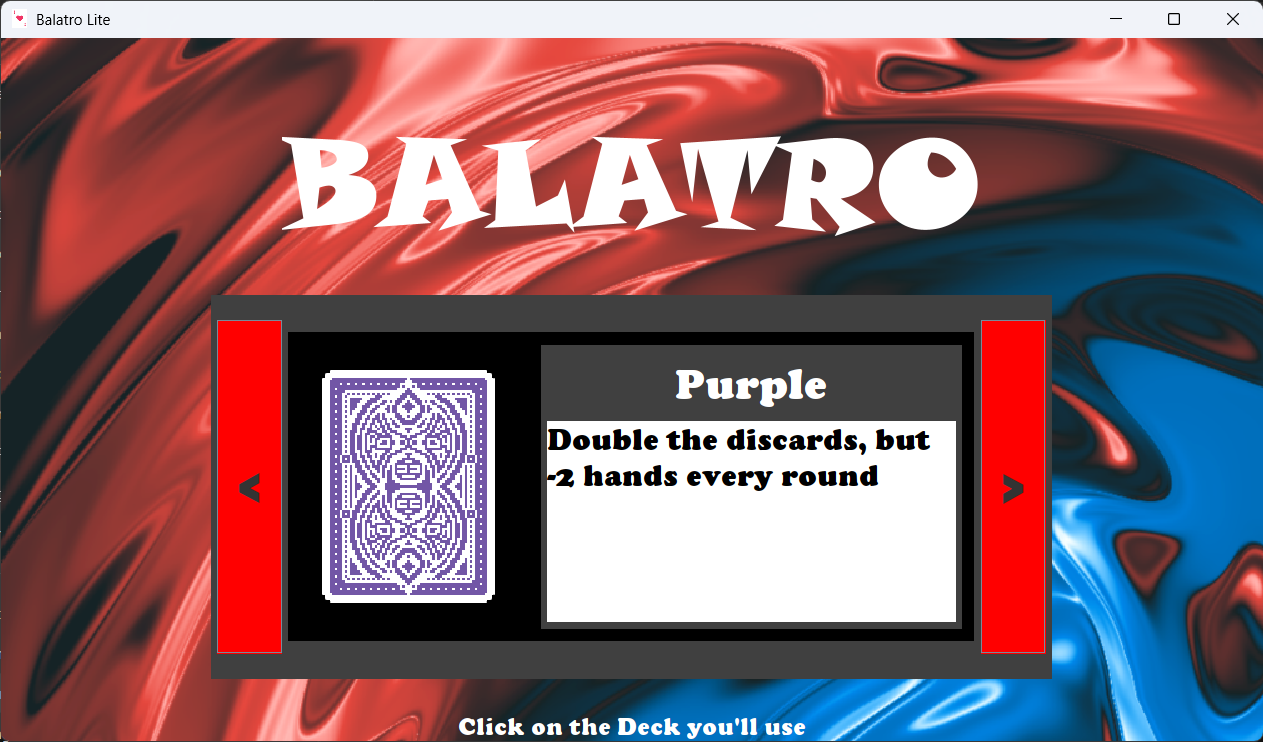
\includegraphics[width=0.8\textwidth]{img/guida/02-DeckChoice}
	\caption{Scelta del Deck}
	\label{img:guida:deck}
\end{figure}

Una volta scelto il mazzo viene caricata l'interfaccia di gioco.

\section{Panoramica dell'Ante}

Prima di iniziare il round, viene sempre visualizzata una panoramica dell'Ante che l'utente dovrà affrontare (\Cref{img:guida:ante}), mostrando i dettagli di ogni Blind che la compongono.

Nel pannello a sinistra vengono visualizzate le informazioni del round corrente.
In particolare nei riquadri mostrati in \Cref{img:guida:infopanel}, vengono riportate le \textbf{mani} e gli \textbf{scarti} rimasti per il round corrente, il \textbf{numero di Ante} che il giocatore ha superato e i \textbf{soldi} che possiede.
Cliccando sul nome del Blind è possibile visualizzarne le caratteristiche.
Cliccando su \textbf{Available Combinations} vengono illustrate le combinazioni riconosciute con relativi punteggi base e moltiplicatori.

Per iniziare la partita vera e propria cliccare il pulsante \textbf{Start Blind}.

\begin{figure}[H]
	\centering{}
	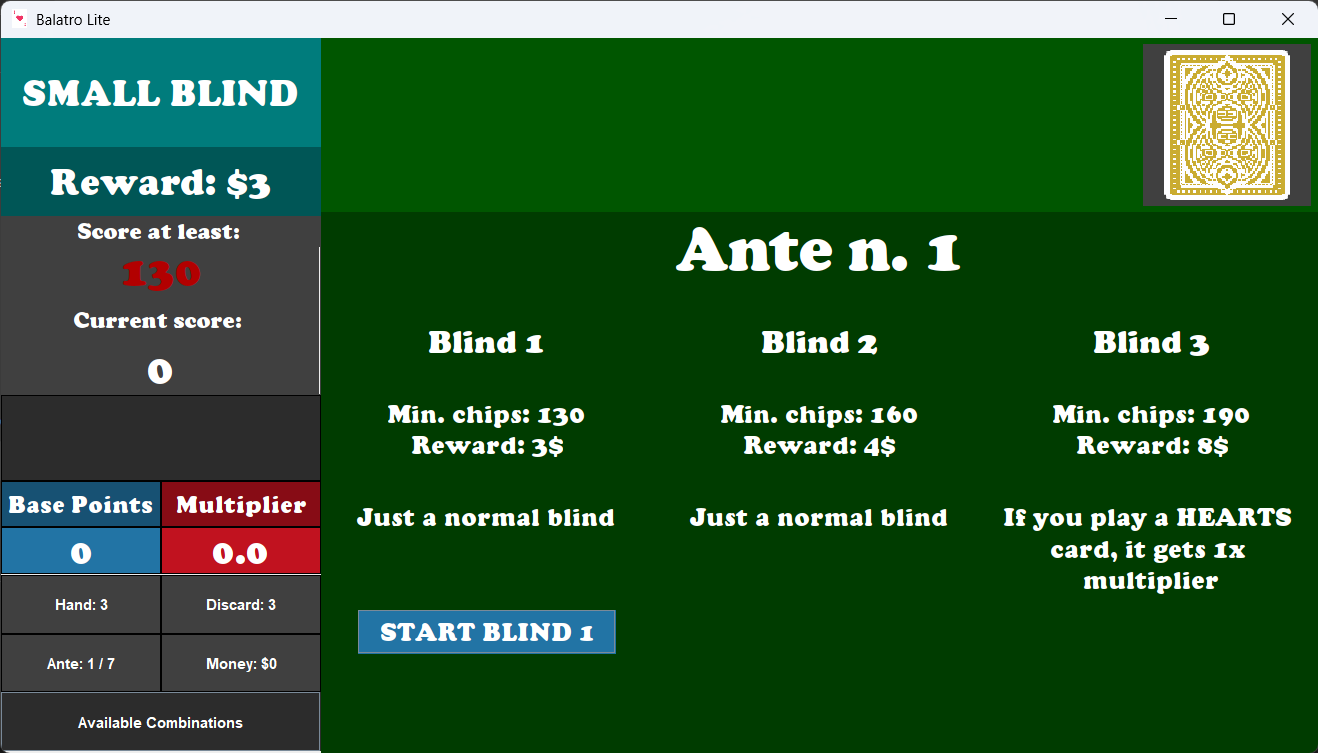
\includegraphics[width=0.8\textwidth]{img/guida/03-AnteView.png}
	\caption{Visualizzazione dell'Ante}
	\label{img:guida:ante}
\end{figure}

\begin{figure}[H]
	\centering{}
	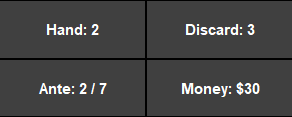
\includegraphics{img/guida/09-InfoPanel}
	\caption{Particolare del pannello informativo}
	\label{img:guida:infopanel}
\end{figure}

\section{Svolgimento di un round}

L'interfaccia di gioco è composta da vari slot (porzioni di interfaccia con sfondo grigio):
\begin{itemize}
    \item Alto a sinistra: contiene i Joker (massimo 5). Cliccando su un Joker è possibile visualizzarne le proprietà e venderlo.
    \item Alto a destra: contiene il mazzo scelto dall'utente. Cliccandolo è possibile visualizzarne le caratteristiche.
    \item Basso: Contiene le carte che il giocatore ha in mano (massimo 7). Cliccandole verranno selezionate perpoterle giocare / scartare.
    \item Centrale: Contiene le carte che il giocatore ha scelto (massimo 5), che potrà giocare o scartare utilizzando gli appositi pulsanti (\textbf{Play Hand} e \textbf{Discard}). Cliccandole vengono rimesse nella mano.
\end{itemize}
È possibile ordinare le carte che il giocatore ha in mano cliccando i pulsanti Sort By \textbf{Rank} / \textbf{Suit}.

\begin{figure}[H]
	\centering{}
	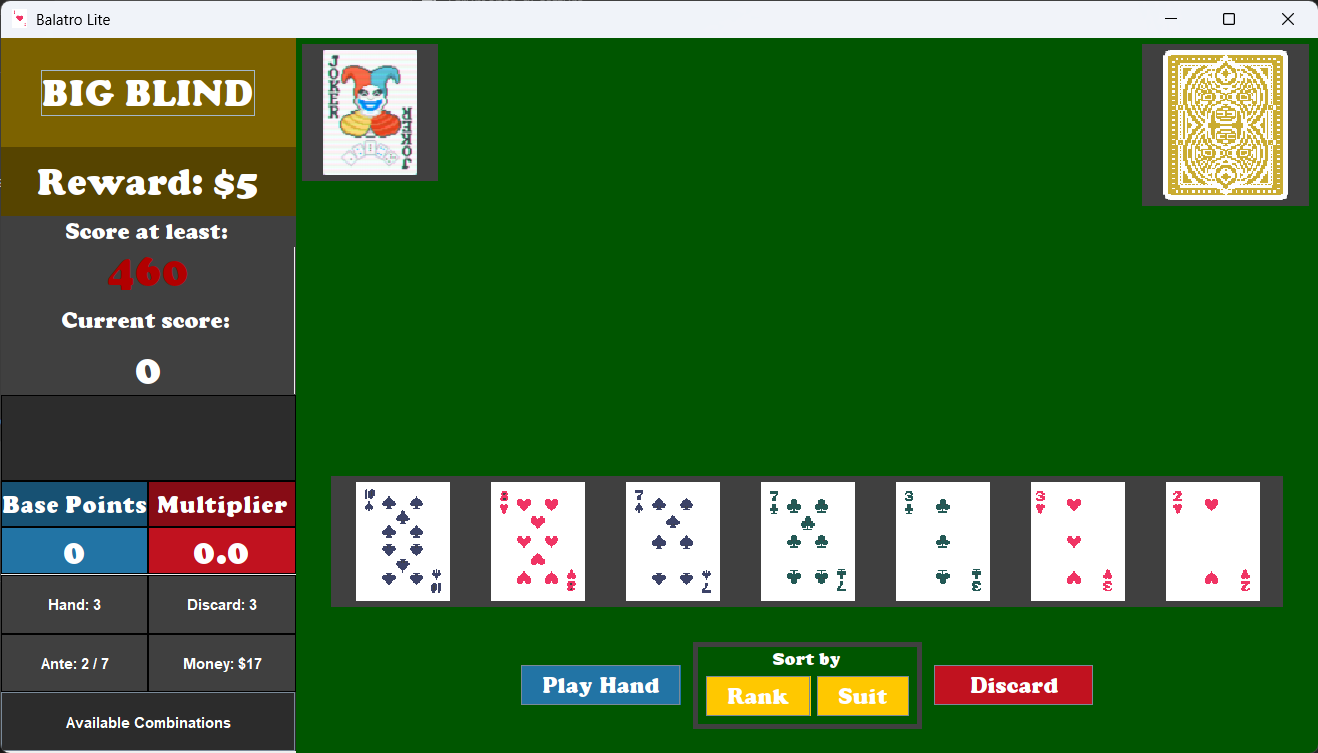
\includegraphics[width=0.8\textwidth]{img/guida/04-GameTable}
	\caption{Tavolo di gioco in cui l'utente ha tutte le carte in mano}
	\label{img:guida:tavolo}
\end{figure}

\begin{figure}[H]
	\centering{}
	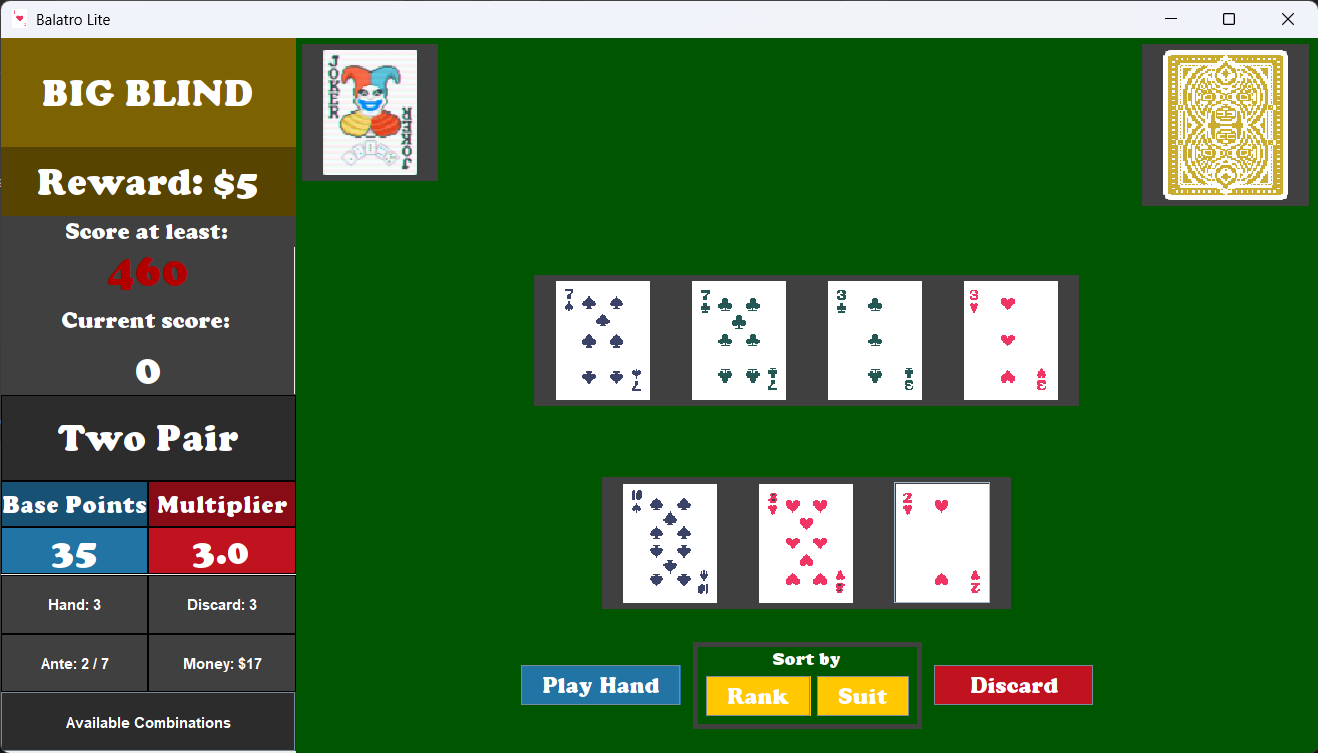
\includegraphics[width=0.8\textwidth]{img/guida/06-CardStaged}
	\caption{Tavolo in cui l'utente ha scelto alcune carte}
	\label{img:guida:cartescelte}
\end{figure}

Quando l'utente sceglie delle carte dalla mano, nel pannello di sinistra viene visualizzata la combinazione data dalle carte selezionate (vedi \Cref{img:guida:cartescelte}).

NB: I dettagli della combinazione non tengono conto di eventuali modifiche date da joker, deck e boss blind. Verranno calcolati solo nel momento in cui viene effettivamente giocata la mano.
Nel caso in cui il giocatore non riesca ad arrivare al numero di chips necessario per sconfiggere il blind, la partita terminerà e verrà chiesto se iniziarne una nuova o uscire dal gioco.
In caso contrario, non appena verrà superata la soglia di chips, il blind sarà considerato superato, e sarà possibile aprire lo shop.

\subsection{Combinazioni riconosciute}
Le combinazioni riconosciute dal gioco sono quelle del Poker, ma vengono di seguito riportate in ordine di importanza decrescente:
\begin{itemize}
	\item \textbf{Scala reale (Royal Flush)}: Una scala da dieci a un asso con cinque carte dello stesso seme.
	\item \textbf{Scala colore (Straight Flush)}: Qualsiasi scala con cinque carte dello stesso seme.
	\item \textbf{Poker (Four of a Kind)}: Quattro carte dello stesso valore.
	\item \textbf{Full (Full House)}: Un tris dello stesso valore + Una coppia di un altro valore.
	\item \textbf{Colore (Flush)}: Cinque carte dello stesso seme.
	\item \textbf{Scala (Straight)}: Cinque carte consecutive di seme diverso.
	\item \textbf{Tris (Three of a Kind)}: Tre carte dello stesso valore.
	\item \textbf{Doppia coppia (Two Pair)}: Due coppie, ognuna composta da due carte dello stesso valore.
	\item \textbf{Coppia (Pair)}: Due carte dello stesso valore.
	\item \textbf{Carta alta (High Card)}: Nessuna delle combinazioni precedenti. Viene presa la singola carta dal valore maggiore.
\end{itemize}
Nelle scale l'Asso può essere utilizzato dopo il K o prima del 2.

\subsection{Esempio di assegnazione dei punteggi}
Il calcolo del punteggio avviene nella seguente maniera - con esempio:
\begin{itemize}
	\item Supponiamo di aver fatto scala da 2 a 6.
	\item Si parte dalla base data dalla combinazione - 20 x 5.
	\item Si aggiungono i rank delle carte, dove ciascuna carta vale:
	\begin{itemize}
		\item esattamente il rank che ha se è minore o uguale a 10 (e.g : 2 vale 2, 3 vale 3, ...).
		\item le carte con figure valgono esattamente 10.
		\item l'asso vale 11 (abbiamo voluto seguire le assegnazioni dei punteggi del gioco originale).
		\item Di conseguenza le carte di questa mano valgono 2 + 3 + 4 + 5 + 6 = 20 --- (20 + 25) x 5.
	\end{itemize}
	\item Si applicano tutti i joker - supponiamo che ci sia un joker da + 10 di moltiplicatore: 45 x 15.
	\item Si applica l'eventuale depotenziamento del blind - con boss che porta il multiplier ad 1: 45 x 1.
	\item Si applica l'eventuale effetto del mazzo - con mazzo gold: 45 x 1 x 2.
	\item A questo punto viene effettuato il calcolo e attributo il punteggio al giocatore - 45 x 1 x 2 = 60 chips.
\end{itemize}



\section{Shop}

Nello shop vengono proposti vari joker: cliccando sul pulsante \textbf{i} ne vengono illustrate le caratteristiche.
Per acquistare un joker è sufficiente cliccarne l'immagine e poi selezionare il pulsante \textbf{Buy}.

Per chiudere lo shop e continuare con la partita cliccare il pulsante \textbf{Continue}.

\begin{figure}[H]
	\centering{}
	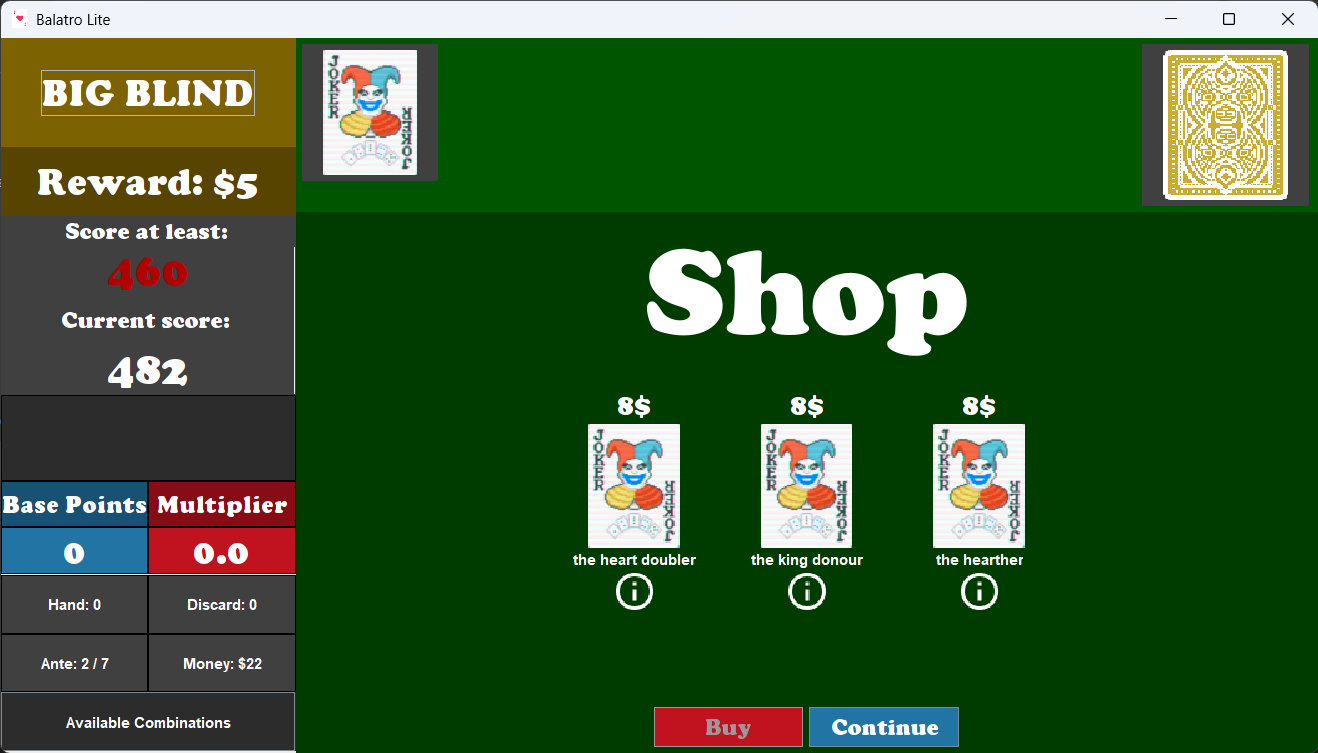
\includegraphics[width=0.8\textwidth]{img/guida/08-Shop}
	\caption{Interfaccia dello Shop in cui è possibile acquistare i Joker}
	\label{img:guida:shop}
\end{figure}

\section{Fine del gioco}

Il gioco continuerà fino al superamento di tutte le Ante, dopo le quali verrà mostrata la schermata di vittoria.


\chapter{Esercitazioni di laboratorio}

\section{enrico.bartocetti@studio.unibo.it}

\begin{itemize}
	 \item Laboratorio 06: \url{https://virtuale.unibo.it/mod/forum/discuss.php?d=176282#p244943}
	 \item Laboratorio 07: \url{https://virtuale.unibo.it/mod/forum/discuss.php?d=177162#p246012}
	 \item Laboratorio 08: \url{https://virtuale.unibo.it/mod/forum/discuss.php?d=178723#p247201}
	 \item Laboratorio 09: \url{https://virtuale.unibo.it/mod/forum/discuss.php?d=179154#p247745}
	 \item Laboratorio 10: \url{https://virtuale.unibo.it/mod/forum/discuss.php?d=180101#p248896}
	 \item Laboratorio 11: \url{https://virtuale.unibo.it/mod/forum/discuss.php?d=181206#p250764}
\end{itemize}

\section{justin.carideo@studio.unibo.it}

\begin{itemize}
	\item Laboratorio 07: \url{https://virtuale.unibo.it/mod/forum/discuss.php?d=177162#p245992}
	\item Laboratorio 08: \url{https://virtuale.unibo.it/mod/forum/discuss.php?d=178723#p247202}
	\item Laboratorio 09: \url{https://virtuale.unibo.it/mod/forum/discuss.php?d=179154#p247752}
	\item Laboratorio 10: \url{https://virtuale.unibo.it/mod/forum/discuss.php?d=180101#p248817}
	\item Laboratorio 11: \url{https://virtuale.unibo.it/mod/forum/discuss.php?d=181206#p250160}
\end{itemize}

\section{nicolas.tazzieri@studio.unibo.it}

\begin{itemize}
	 \item Laboratorio 07: \url{https://virtuale.unibo.it/mod/forum/discuss.php?d=177162#p246162}
	 \item Laboratorio 09: \url{https://virtuale.unibo.it/mod/forum/discuss.php?d=179154#p248370}
	 \item Laboratorio 10: \url{https://virtuale.unibo.it/mod/forum/discuss.php?d=180101#p249656}
	 \item Laboratorio 11: \url{https://virtuale.unibo.it/mod/forum/discuss.php?d=181206#p250849}
\end{itemize}

\section{nicholas.benedetti@studio.unibo.it}

\begin{itemize}
    \item Laboratorio 09: \url{https://virtuale.unibo.it/mod/forum/discuss.php?d=179154#p248189}
\end{itemize}

\end{document}


